\documentclass[13pt,a4paper]{extarticle}
\usepackage[utf8]{inputenc}
\usepackage[utf8]{vietnam} %Bien dich duoc tieng Viet
\usepackage{amsmath,amsfonts,amssymb} %Font toan
\usepackage{type1cm}
\usepackage{times}
\usepackage{graphicx}
\graphicspath{ {images02/} }
\usepackage{enumerate}
\usepackage{comment}
\usepackage{multicol}
\usepackage{multirow}
%\usepackage[unicode]{hyperref} %Tu dong tao bookmark
\usepackage[unicode, hidelinks=true]{hyperref}
\usepackage{indentfirst} %Thut vao dau dong o tat ca cac doan
\usepackage{listings} %Dinh dang code
\usepackage{color} %Mau sac
\usepackage[left=2.5cm,right=2.5cm,top=2.5cm,bottom=2.5cm]{geometry} %Canh lề trái - phải - trên - dưới cho tài liệu
\usepackage{longtable}
\renewcommand{\arraystretch}{1.3}

\begin{document}
\pagenumbering{gobble}
\title{\Large{\textbf{BÀI CHUẨN BỊ THỰC TẬP ĐIỆN CÔNG NGHIỆP}}\\\vspace{1cm}\textbf{Bài 2}\\\vspace{.5cm}\textbf{XÁC ĐỊNH CỰC TÍNH, VẬN HÀNH CÁC LOẠI ĐỘNG CƠ KĐB 1 PHA, 3 PHA 6, 9 ĐẦU DÂY}}
\date{Ngày 26 tháng 05 năm 2016}
%\date{\today}
\author{GVHD: Thầy Võ Minh Thiện \vspace{.6cm}\\  Nhóm SVTH: Nhóm 2 -- Tiểu nhóm 1: Thi Minh Nhựt}
\maketitle
\tableofcontents
\newpage
\pagenumbering{arabic}
\setcounter{page}{1}
\section{Chuẩn bị}
Gồm có: VOM kim, pin 9V, băng keo, bút, giấy đánh số xác định đầu cuối của cuộn dây, mô hình vận hành động cơ, đòng hồ đo dòng và áp.
\section{Động cơ điện một pha bốn đầu dây chạy tụ khởi động (tụ đề)}
\subsection{Xác định cuộn chạy và cuộn đề}
\label{sec:chay-tu-de}
\begin{figure}[!h]
\begin{center}
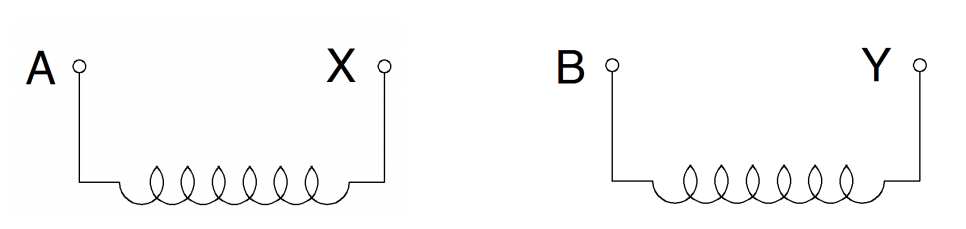
\includegraphics[scale=.5]{1p-4day}
\end{center}
\caption{Xác định cực tính của động cơ 1 pha 4 đầu dây}
\end{figure}

Thực hiện thao các bước sau:
\begin{list}{--}{}
\item Dùng VOM đo 2 đầu dây bất kỳ (thang đo $\times 1$).
\item Nếu cùng một cuộn dây thì sẽ có điện trở: ghi nhận lại các giá trị điện trở.
\item Nếu cuộn nào có \emph{điện trở nhỏ hơn} là cuộn chạy.
\item Cuộn còn lại là cuộn chạy.
\end{list}
\subsection{Sơ đồ đấu dây chạy tụ khởi động}
\begin{figure}[!h]
\begin{center}
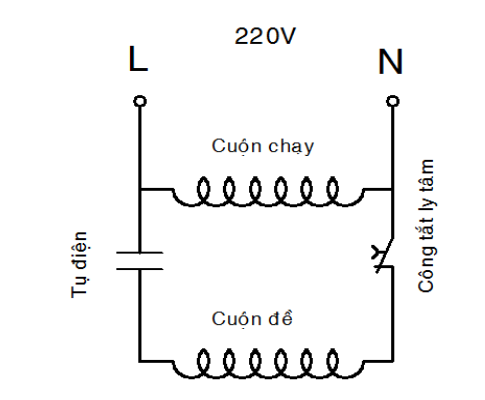
\includegraphics[scale=.45]{chay-de-1}
\end{center}
\caption{Sơ đồ đấu dây chạy tụ khởi động}\label{Fig:chay-de-1}
\end{figure}
\subsection{Vận hành động cơ một pha chạy tụ khởi động}
Thực hiện theo các bước:
\begin{list}{--}{}
\item \textit{Bước 1}: Đấu các cuộn dây của động cơ như hình~\ref{Fig:chay-de-1}.
\item \textit{Bước 2}: Đấu mạch điều khiển như hình~\ref{Fig:mach-dieu-khien-1p-tu-de}.
\begin{figure}[!h]
\begin{center}
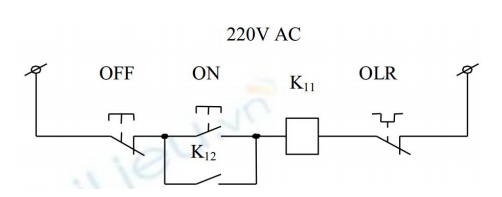
\includegraphics[scale=.6]{van-hanh-1p-tu-de-1}
\end{center}
\caption{Mạch động cơ một pha}\label{Fig:mach-dieu-khien-1p-tu-de}
\end{figure}
\item \textit{Bước 3}: Đấu mạch động lực như hình~\ref{Fig:mach-dong-luc-1p-tu-de}.
\begin{figure}[!h]
\begin{center}
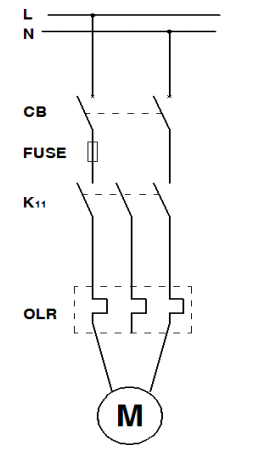
\includegraphics[scale=.6]{van-hanh-1p-tu-de}
\end{center}
\caption{Mạch động lực vận hành động cơ một pha}\label{Fig:mach-dong-luc-1p-tu-de}
\end{figure}
\item \textit{Bước 4}: Nhờ GVHD kiểm tra cho phép vận hành.
\item \textit{Bước 5}: Bật CB, nhấn nút ON, ghi nhận lại các giá trị sau:
\begin{center}
\begin{tabular}{|c|c|c|c|c|}\hline
\textit{Động cơ} & $U_{\text{\textit{vận hành}}}, V$ & $I_{\text{\textit{khởi động}}}, A$ & $I_{\text{\textit{không tải}}}, A$ & $P_{\text{\textit{không tải}}}, W$ \\ \hline
Chạy tụ đề & & & & \\ \hline
& & & & \\ \hline
& & & & \\ \hline
Chạy tụ ngậm & & & & \\ \hline
& & & & \\ \hline
& & & & \\ \hline
\end{tabular}
\end{center}
\item \textit{Bước 6}: Dựa vào thông số trên nhãn động cơ, xác định công suất động cơ.
\item \textit{Bước 7}: Nhấn nút OFF, tháo động cơ chạy tụ đề và thay động cơ chạy tụ ngậm vào vận hành. Chú ý, đấu dây lại cho động cơ chạy tụ ngậm như hình~\ref{Fig:chay-ngam-1}.
\item \textit{Bước 8}: Lặp lại \textit{bước 4} đến \textit{bước 7}.
\end{list}
\section{Động cơ điện một pha 4 đầu dây chạy tụ ngậm (động cơ 2 pha)}
\subsection{Xác định cực tính}
Thực hiện tương tự như mục~\ref{sec:chay-tu-de}.
\subsection{Sơ đồ đấu dây chạy tụ ngậm}
\begin{figure}[!h]
\begin{center}
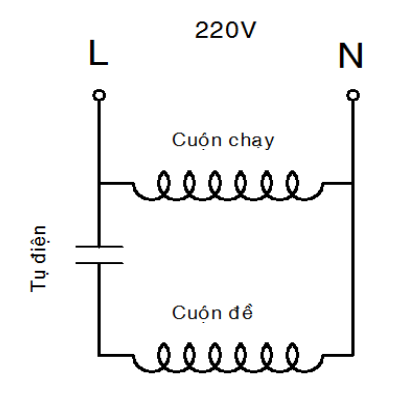
\includegraphics[scale=.5]{chay-ngam-2}
\end{center}
\caption{Sơ đồ đấu dây chạy tụ ngậm}\label{Fig:chay-ngam-1}
\end{figure}
\section{Động cơ 3 pha 6 đầu dây}
\subsection{Xác định cực tính của động cơ 3 pha 6 đầu dây}
Việc xác định cực tính là rất quan trọng.
\begin{figure}[!h]
\begin{center}
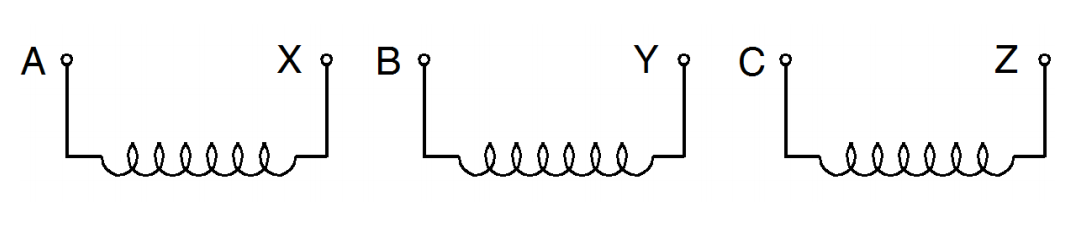
\includegraphics[scale=.6]{3p-6day}
\end{center}
\caption{Xác định cực tính của động cơ 3 pha 6 đầu dây}
\end{figure}

Thực hiện theo các bước sau:
\begin{list}{--}{}
\item \textit{Bước 1}: Dùng VOM (thang $\times 1 \Omega$) xác định 2 đầu dây của một cuộn dây. Gọi các cuộn lần lượt là $AX, BY, CZ$.

Ở bước này, ta chưa xác định được đầu cuối của cuộn dây
\item \textit{Bước 2}: Đánh dấu số thứ tự cho 2 đầu dây của các cuộn: $AX \longleftrightarrow 12$, $BY \longleftrightarrow 34$ và $CZ \longleftrightarrow 56$.
\item \textit{Bước 3}: Mắc 2 đầu của một cuộn dây vào 2 đầu của pin 9V thông qua \textit{công tắc}, chuyển VOM sang thang đo $mA$:
\begin{list}{+}{}
\item Giả sử: $AX = 12$, cần xác đinh cặp $34 = ??$
\item Đặt que đen: số 3; que đỏ: số 4. Đóng công tắc.
\item Nếu kim quay theo chiều thuận và về 0 thì: $34=BY$, ngược lại thì $34 = YB$.
\item Xác định cặp $56 = ??$, thực hiện tương tự.
\item[$\Longrightarrow$] Vì quá trình đóng công tắc thì dòng điện mới biến thiên (xảy ra quá trình quá độ trong mạch). Giải thích trong sơ đồ hình~\ref{Fig:qua-do}
\begin{figure}[!h]
\begin{center}
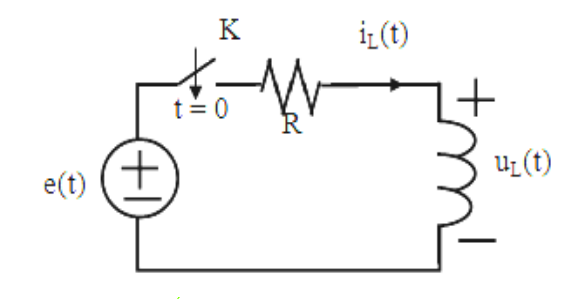
\includegraphics[scale=.5]{quado-1}
\end{center}
\caption{Quát trình quá độ với cuộn dây}\label{Fig:qua-do}
\end{figure}

Khi đó, dòng điện $\displaystyle i\left({t}\right) = Ke^{-\frac{R}{L}t} \longrightarrow 0$
\end{list}
\item \textit{Bước 4}: Đánh dấu lại các cực tính vừa xác định được.
\end{list}
\newpage
\subsection{Sơ đồ đấu dây động cơ 3 pha kiểu Y}
\begin{figure}[!h]
\begin{center}
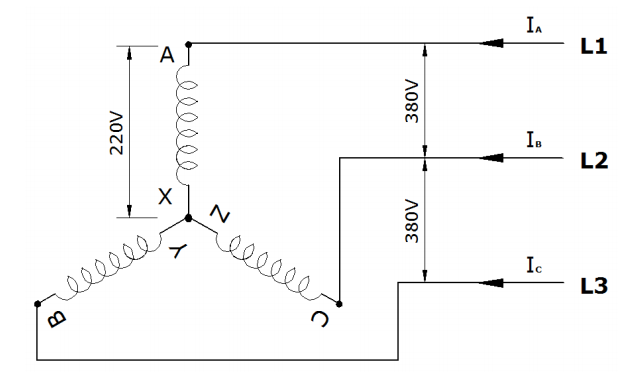
\includegraphics[scale=.5]{dau-day-3-pha-Y.png} 
\end{center}
\caption{Sơ đồ đấu dây động cơ 3 pha kiểu Y}\label{Fig:dc-3p}
\end{figure}
\subsection{Vận hành động cơ 3 pha}
Thực hiện theo các bước sau:
\begin{list}{--}{}
\item \textit{Bước 1}: Đấu các cuộn dây của động cơ như hình~\ref{Fig:dc-3p}.
\item \textit{Bước 2}: Nối đất thiết bị.
\item \textit{Bước 3}: Đấu mạch điều khiển như hình~\ref{Fig:mach-dieu-khien-3p}.
\begin{figure}[!h]
\begin{center}
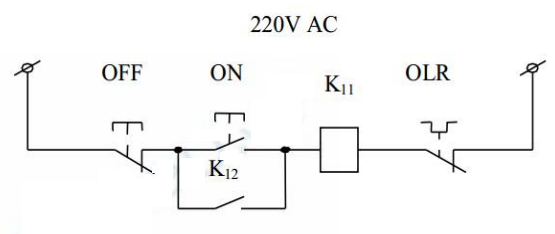
\includegraphics[scale=.6]{van-hanh-3p-1}
\end{center}
\caption{Mạch động cơ ba pha}\label{Fig:mach-dieu-khien-3p}
\end{figure}
\item \textit{Bước 4}: Đấu mạch động lực như hình~\ref{Fig:mach-dong-luc-3p}.
\begin{figure}[!h]
\begin{center}
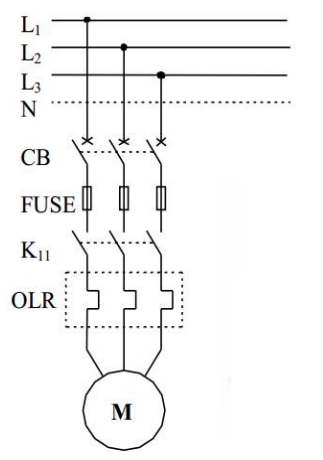
\includegraphics[scale=.6]{van-hanh-3p}
\end{center}
\caption{Mạch động lực vận hành động cơ ba pha}\label{Fig:mach-dong-luc-3p}
\end{figure}
\item \textit{Bước 5}: Nhờ GVHD kiểm tra cho phép vận hành.
\item \textit{Bước 6}: Bật CB, nhấn nút ON, ghi nhận lại các giá trị sau:
\begin{center}
\begin{tabular}{|c|c|c|c|}\hline
$U_{\text{\textit{vận hành}}}, V$ & $I_{\text{\textit{khởi động}}}, A$ & $I_{\text{\textit{không tải}}}, A$ & $P_{\text{\textit{không tải}}}, W$ \\ \hline
$U_{AB} = $& $I_A = $& $I_A = $& \\ \hline
& & & \\ \hline
$U_{BC} = $& $I_B = $& $I_B = $& \\ \hline
& & & \\ \hline
$U_{AC} = $& $I_C = $& $I_C = $& \\ \hline
& & & \\ \hline
\end{tabular}
\end{center}
\item[$\ast$] Giá trị $P_0$ dựa vào công suất ghi trên nhãn máy.
\item \textit{Bước 7}: Nhấn nút OFF, tháo mạch kết thúc thực tập.
\item \textit{Bước 8}: Vệ sinh, tháo mạch và sơ đồ trả lại cũ.
\end{list}
\begin{comment}
\section{Trả lời câu hỏi}
\begin{enumerate}[{\it 1.}]
\item \textit{Mục đích của việc xác định cực tính của động cơ?}

Là để đấu dây vận hành động cơ, khi không xác định được cực tính thì đấu dây vận hành xác suất hỏng động cơ là rất cao.
\item \textit{So sánh động cơ 1 pha và 3 pha. Nêu ứng dụng}
\begin{list}{--}{}
\item Khi cùng một công suất thì động cơ 3 pha khởi động tốt hơn, momen ổn định hơn và hiệu suất cao hơn.
\end{list}
\end{enumerate}
\end{comment}
\section{Bài thực tập thêm}
\paragraph{Yêu cầu}Đấu dây động cơ không đồng bộ 3 pha thành động cơ 1 pha.
\paragraph{Thực hiện}
\begin{list}{--}{}
\item Cách đấu dây động cơ 3 pha không thay đổi.
\item Điện áp định mức mỗi pha phải phù hợp với điện áp nguồn cung cấp.
\item Cường độ dòng điện trong mỗi pha phải tương đối bằng nhau và không lớn hơn cường độ định mức trong cuộn pha khi động cơ đang vận hành có tải.
\item Tăng lực khởi động: $C_{\text{\textit{kđ}}} = \left({2.5 \div 3}\right)C_{lv}$.
\item Công suất còn lại: $P = \left({0.6 \div 0.75}\right)P_{3p}$.
\item Tụ làm việc: $\displaystyle C_{lv} = 1600\times \frac{I_p}{U_p}~[MF]$.
\item Điện áp tụ làm việc: $U_C = 2U$.
\end{list}
\paragraph{Sơ đồ đấu dây} hình~\ref{Fig:3p-1p}.
\begin{figure}[!h]
\begin{center}
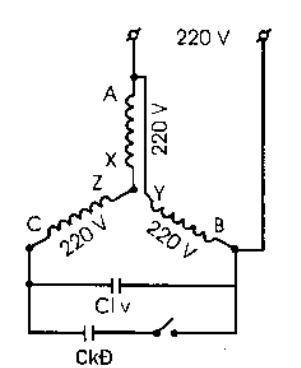
\includegraphics[scale=.6]{3p-1p}
\end{center}
\caption{Đấu dây động cơ 3 pha thành động cơ 1 pha}
\label{Fig:3p-1p}
\end{figure}
\newpage
\paragraph{Mạch động lực} hình~\ref{Fig:3p-1p-dong-luc}.
\begin{figure}[!h]
\begin{center}
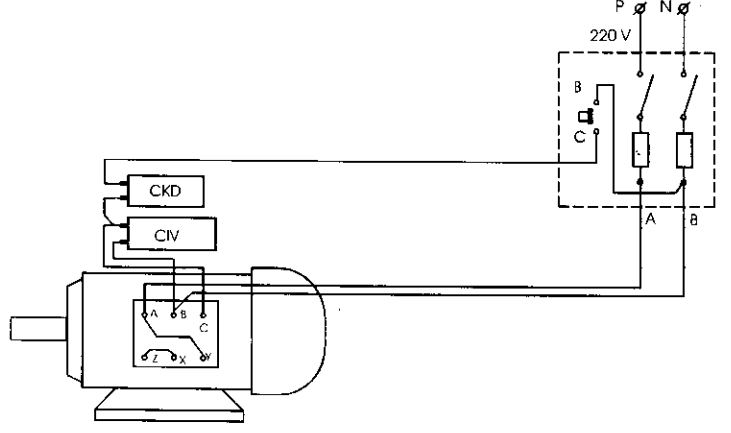
\includegraphics[scale=.5]{3p-1p-dong-luc}
\end{center}
\caption{Mạch động lực đấu 3 pha thành 1 pha}
\label{Fig:3p-1p-dong-luc}
\end{figure}
\end{document}